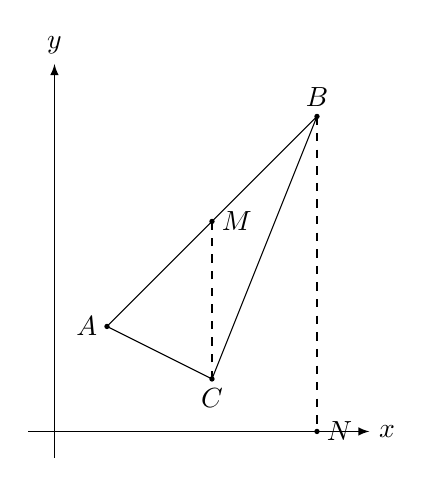
\begin{tikzpicture}[scale=0.6667,>=latex]
  \draw[->] (-0.5,0)--(6,0) node[right]{$x$};
  \draw[->] (0,-0.5)--(0,7) node[above]{$y$};
  \coordinate (A) at (1,2);
  \coordinate (B) at (5,6);
  \coordinate (C) at (3,1);
  \coordinate (M) at (3,4);
  \coordinate (N) at (5,0);
  \draw (A)--(B)--(C)--cycle;
  \draw[dashed] (C)--(M);
  \draw[dashed] (B)--(N);
  \fill (A) circle(1.45pt) node[left]{$A$};
  \fill (B) circle(1.45pt) node[above]{$B$};
  \fill (C) circle(1.45pt) node[below]{$C$};
  \fill (M) circle(1.45pt) node[right]{$M$};
  \fill (N) circle(1.45pt) node[right]{$N$};
\end{tikzpicture}
